\section{Call Graphs}
\label{section:unsorted/call_graphs}

With a project the size of PLOP it becomes difficult for developers to understand the flow of the program.
At the moment there are over thirteen thousand different subroutines in more than 750 different source files.
The problem of ?? especially with the high turnover intrinsic to an academic lab.


One popular analysis tool to help in the analysis of a large problem such as this is a call graph \cite{graham1982gprof}.
This is a directed graph representing the call stack for each function or subroutine in a program.

In order to make analysis of PLOP 


\begin{figure}[h]
    \centering
    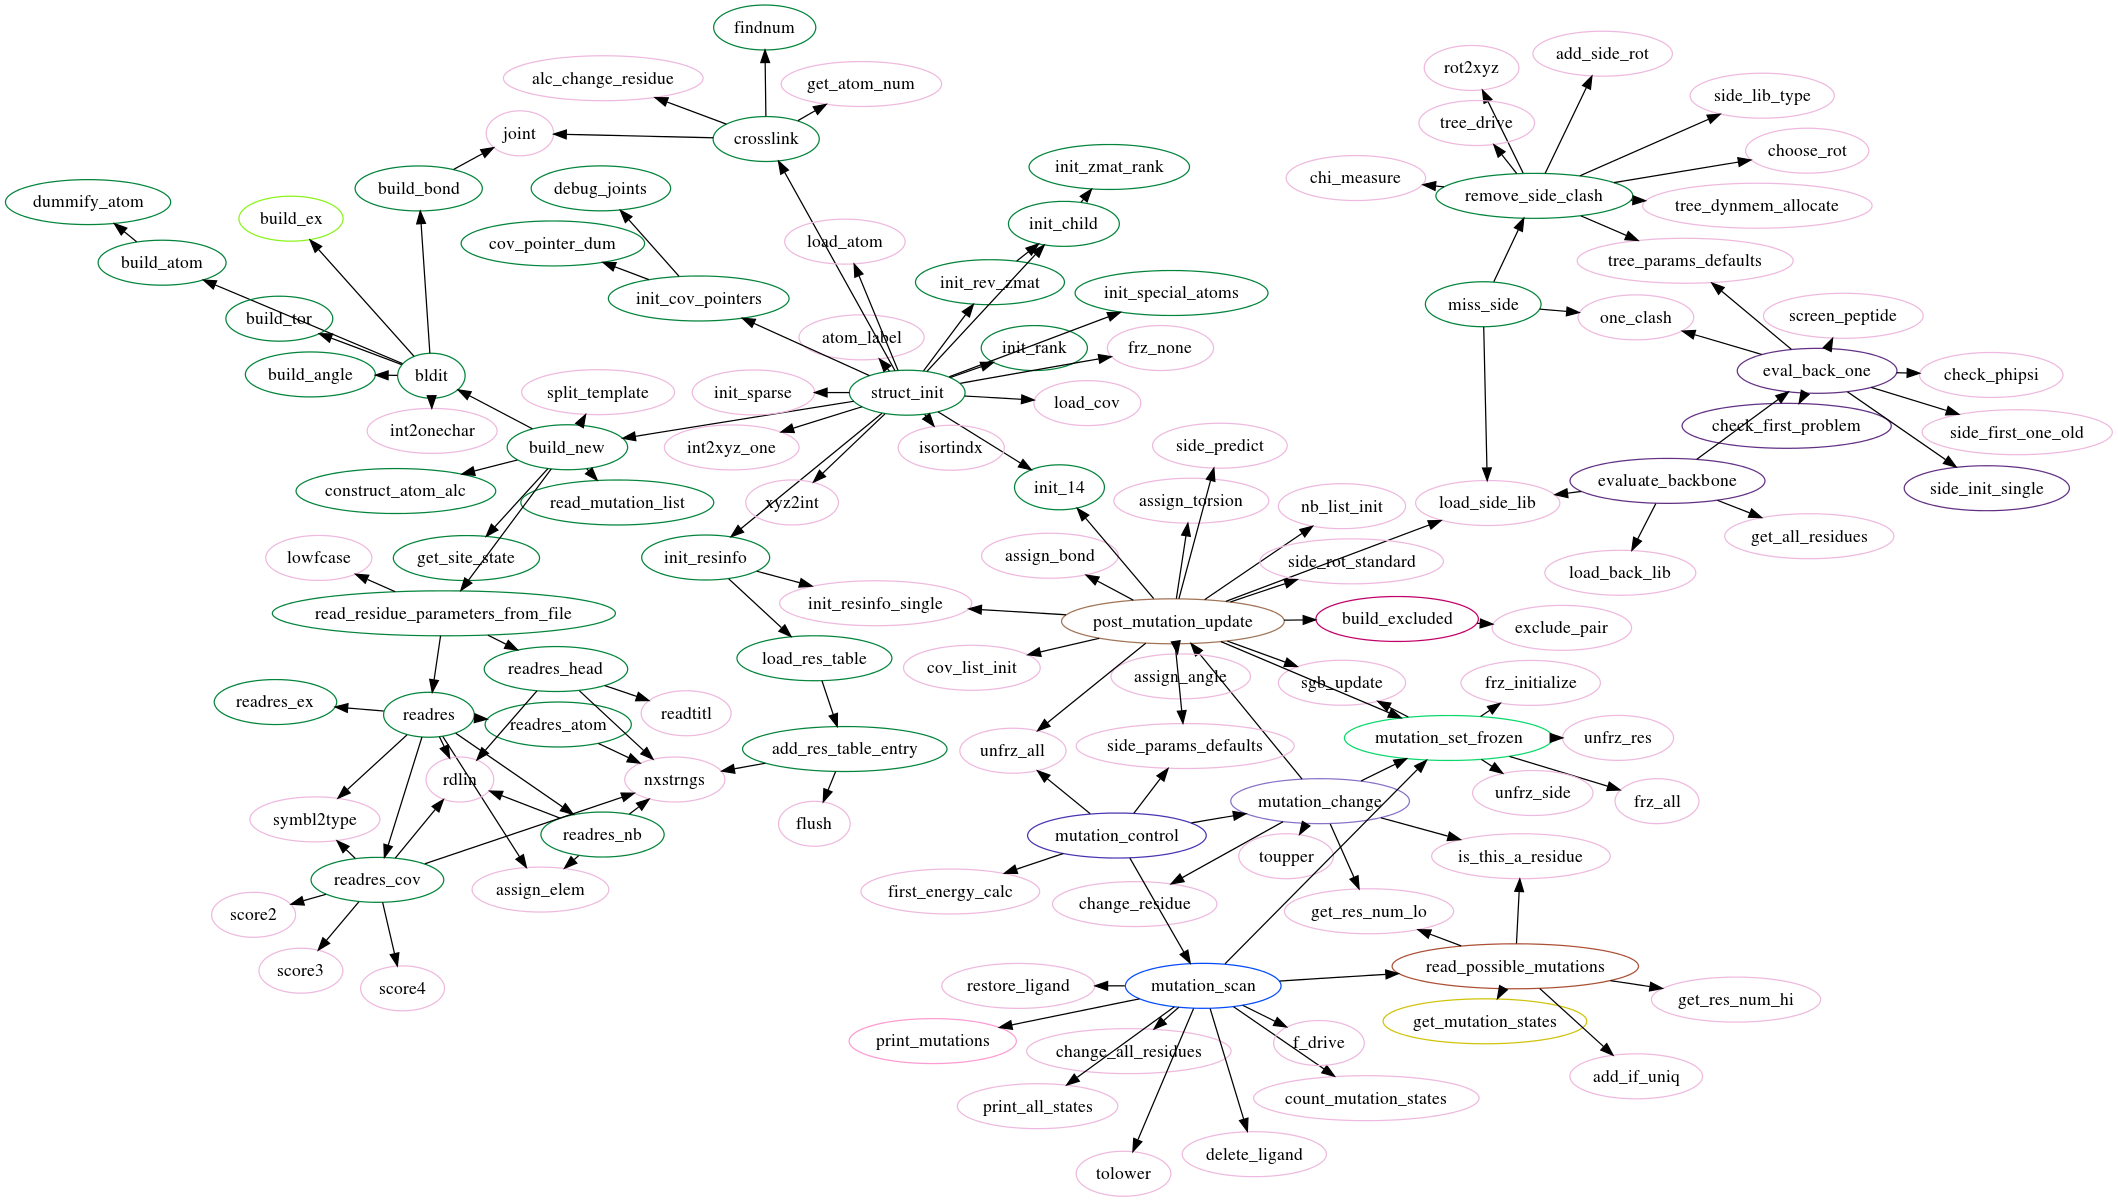
\includegraphics[width=1.0\textwidth,height=0.9\textheight,keepaspectratio]{figures/plop_connected_sfdp.png}
    \caption{An example call graph generated for for the code implementing mutation scanning and certain files having to do with building a structure in memory.}
    \label{figure:mutation_call_graph}
\end{figure}

